\documentclass{myreport}


\usepackage[alf,bibjustif,abnt-emphasize=bf]{abntex2cite} % Estilo das referências

%\setfigdir{img}

\hyphenation{par-ti-cu-lar}
%%%%%%%%%%%%%%%%%%%%%%%%%%%%%%%%%%%%
\hypersetup{
colorlinks = {true},
linktocpage = {false},
plainpages = {false},
linkcolor = {Blue},
citecolor = {Blue},
urlcolor = {Blue},
unicode = {true},
pdftitle = {Machine Learning I},
pdfauthor = {Augusto Ícaro Farias da Cunha},
pdfsubject = {Relatório de estudos},
pdfkeywords={Machine Learning, Deep Learning, Multi Layer Perceptron, Convolutional Neural Network},
pdfcreator = {LaTeX2e},
pdffitwindow = {false},
pdfstartview = {FitH},
pdftoolbar = {true},
pdfpagemode = {UseOutlines},
pdfview = {XYZ null null null}
}
%%%%%%%%%%%%%%%%%%%%%%%%%%%%%%%%%%%%%

\autor{Aluno}{aluno@ic.ufal.br}{matricula}{Ciência da Computação}{7°}

\empresa{Empresa}{Supervisor}{N registro}

\estagio{01/06/2021}{01/12/2021}{20}{200}{5 meses}

\cidade{Maceió - AL}

\ano{2021}

\begin{document}
\newgeometry{top=2.5cm,bottom=2.5cm,left=3cm,right=2cm,heightrounded}
\capa
\folhaDeRosto
\newgeometry{top=2.5cm,bottom=2.5cm,left=3cm,right=2cm,includefoot,heightrounded}
\newpage
\tableofcontents
\newpage
% \listoffigures\thispagestyle{fancy}
% \addcontentsline{toc}{section}{Lista de Figuras}
% \newpage
% \lstlistoflistings\thispagestyle{fancy}
% \addcontentsline{toc}{section}{Lista de Códigos}
% \newpage
% \listoftables\thispagestyle{fancy}
% \addcontentsline{toc}{section}{Lista de Tabelas}
\inicio
\chapter{Introdução}
Descrever o Local de Estágio; o público atendido; os serviços oferecidos; os produtos elaborados; os tipos de materiais que compõem o acervo; a organização e disposição do espaço físico; a equipe; as funções ou atividades exercidas pelos membros da equipe.

\chapter{Atividades Desenvolvidas}
Descrever sobre as atividades desenvolvidas pelo estagiário; os procedimentos desenvolvidos como prática de estágio; os instrumentos adotados para acompanhamento e avaliação das atividades do estagiário; material bibliográfico colocado à disposição para estudo do estagiário; o tipo e a forma de orientação dada ao estagiário pelo supervisor local.

\chapter{Suporte Teórico Para a Solução de Problemas}
Discorrer sobre a bibliografia utilizada enquanto estagiário para solucionar problemas identificados durante o estágio, e referenciá-la. Seguindo normas da ABNT.

\chapter{Conclusão}
Comentar se o estágio realizado foi satisfatório, como sentiu o contato com os futuros colegas de profissão.

Fazer uma correlação entre o estágio prático e os conhecimentos teóricos adquiridos nas disciplinas relacionadas e no material de referência bibliográfica.


\chapter{Anexos}
https://ufal.br/estudante/graduacao/estagios/documentos\cite{UFAL}

Anexar as Avaliações do Supervisor, conforme o modelo disponibilizado no MGE;

Anexar cópia do termo de compromisso, com assinatura do(a) Coordenador(a) de Estágios.

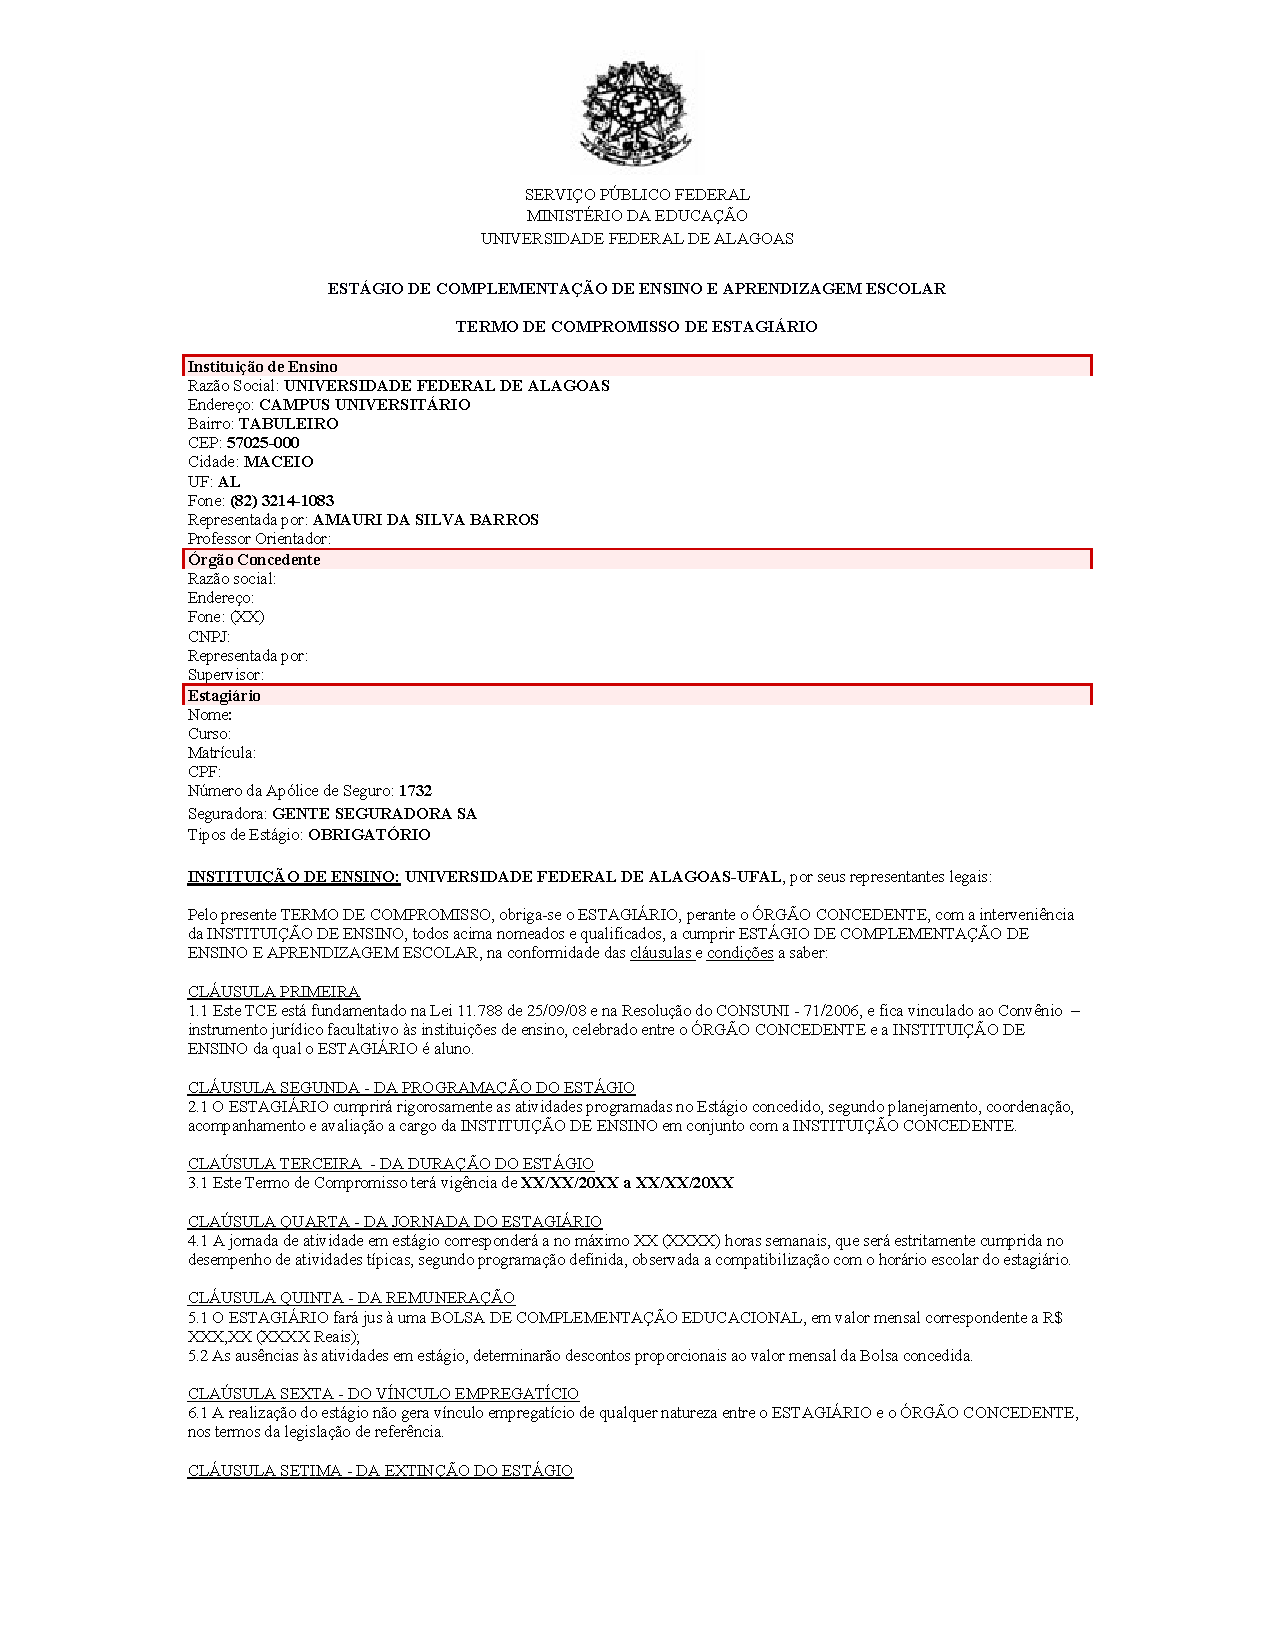
\includepdf[pages=-,pagecommand={},height=\textheight]{tce}

\chapter{De Acordo}
\vfill
\begin{tabular}{>{\centering\arraybackslash} m{6cm} >{\centering\arraybackslash} m{1cm} >{\centering\arraybackslash} m{6cm}}
\hrulefill & e & \hrulefill \\
Carimbo e assinatura do & & Nome completo do \\
Supervisor & & Estagiário \\
\end{tabular}
\vfill



\clearpage
%------------------------------------------------------------------------------
% Gera o índice remissivo do documento
%------------------------------------------------------------------------------
% \newpage
%\begin{appendices}
% \chapter{Extras}
% Neste capítulo compartilho parte das funções principais em python usadas para gerar este relatório.
% \section{Matriz de confusão}
% \lstinputlisting[label=lst:cm,title=Função de geração da matriz de confusão,caption=Função de geração da matriz de confusão]{codes/confusionMatrix.py}
%\end{appendices}

%------------------------------------------------------------------------------
% REFERÊNCIAS BIBLIOGRÁFICAS UTILIZADAS NO TRABALHO
%------------------------------------------------------------------------------
\bibliography{ref}

\end{document}
